\documentclass{jlreq}
\usepackage{url,graphicx,hyperref}

\title{電気電子工学実験3 テーマE(b) \\ ライフゲームの製作}
\author{三木 健太郎}
\date{2024年2月12日}

\begin{document}
\maketitle

\section{制作物の概要}
本実験の自由製作では、ライフゲームのシミュレーションの様子を32×32のマトリクスLED上に表示するデバイスを製作した。また、シミュレーションの初期状態の設定、シミュレーションの開始、リセットを行える操作画面も別途実装した。この操作画面は、マイコン(Raspberry Pi Pico W)と同じネットワークに接続しているコンピュータのWebブラウザからアクセスすることができる。

\begin{figure}[h]
    \begin{center}
        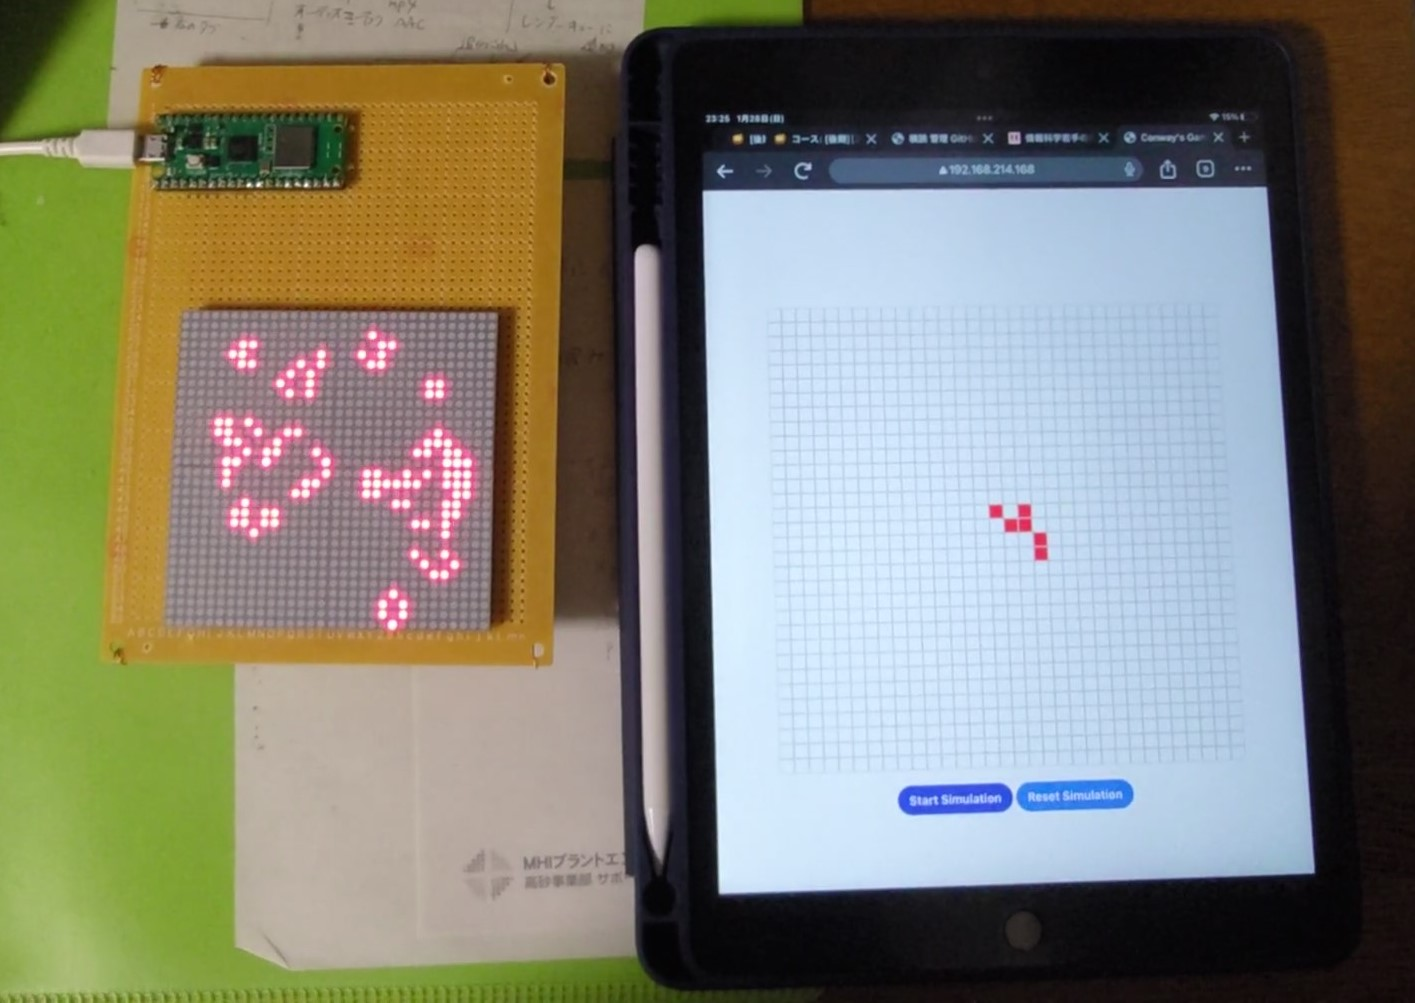
\includegraphics[width=120mm]{img/life-game-indicator.jpg}
    \end{center}
    \caption{制作物の概要}
    \label{img:overall}
\end{figure}

\section{ライフゲームとは}
ライフゲームは、イギリスの数学者John Horton Conwayが考案した数理モデルであり、生命の誕生、成長、消滅といった現象を簡易にシミュレーションするものである。ライフゲームでは、まず二次元の格子上に生きているセルを配置し、以下のルールに従いセルの生死を更新していく。この過程を繰り返すことで、セルの配置が時間とともに変化していく様子を観察することができる。

\begin{description}
    \item[誕生] 死んでいるセルに生きているセルが3つ隣接していれば、次世代でそのセルは生存
    \item[生存] 生きているセルに生きているセルが2つか3つ隣接していれば、次世代でもそのセルは生存
    \item[過疎] 生きているセルに隣接する生きたセルが1つ以下であれば、次世代でそのセルは死滅
    \item[過密] 生きているセルに生きたセルが4つ以上隣接していれば、次世代でそのセルは死滅
\end{description}

\begin{figure}[h]
    \begin{center}
        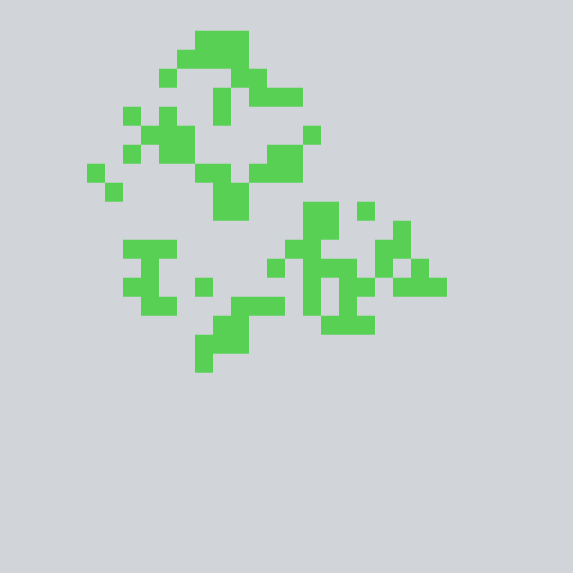
\includegraphics[width=60mm]{img/lifegame.png}
    \end{center}
    \caption{ライフゲームのシミュレーションの様子}
    \label{img:lifegame}
\end{figure}

\section{実装の詳細}
\subsection{材料}
\begin{itemize}
    \item 32×16マトリクスLEDモジュール\footnote{\url{https://eleshop.jp/shop/g/gK4U419/}} 2個
    \item Raspberry Pi Pico W
    \item ユニバーサル基板
    \item エナメル線
\end{itemize}
Raspberry Pi Pico W は、RP2040を搭載したマイコンボードであり、Arduino IDEでの開発が可能である。このマイコンボードはWiFiの通信モジュールを搭載しており、ネットワークを用いたデバイスを容易に製作できる。

\subsection{実装方法}
まず、ハードウェアの実装について述べる。先述のマトリクスLEDモジュールは、制御用のICや周辺回路を含め、1つの基板上に実装されていた。今回は2つのマトリクスLEDを縦に並べて利用するために、マトリクスLEDを元々実装されていた基板から切り離し、ユニバーサル基板上に並べて使用した。

次にソフトウェアの実装について述べる。ソースコードは、ライフゲームのシミュレーションを行う\verb|life-game.ino|、マトリクスLEDの制御を行うプログラム\verb|digit_matrix_led.ino|、操作画面用のWebサーバを立ち上げる\verb|http_server.ino|、これらのプログラムをまとめる\verb|main.ino|の4つのファイルから構成されている。\verb|Raspberry Pi Pico W|をHTTPサーバとして動作させ、Webブラウザからリクエストを受け取ると、ライフゲームのシミュレーションの開始、リセットを行うようになっている。なお、実装したプログラムはGitHub(\url{https://github.com/mikiken/life-game/})で公開している。

\begin{figure}[h]
    \begin{center}
        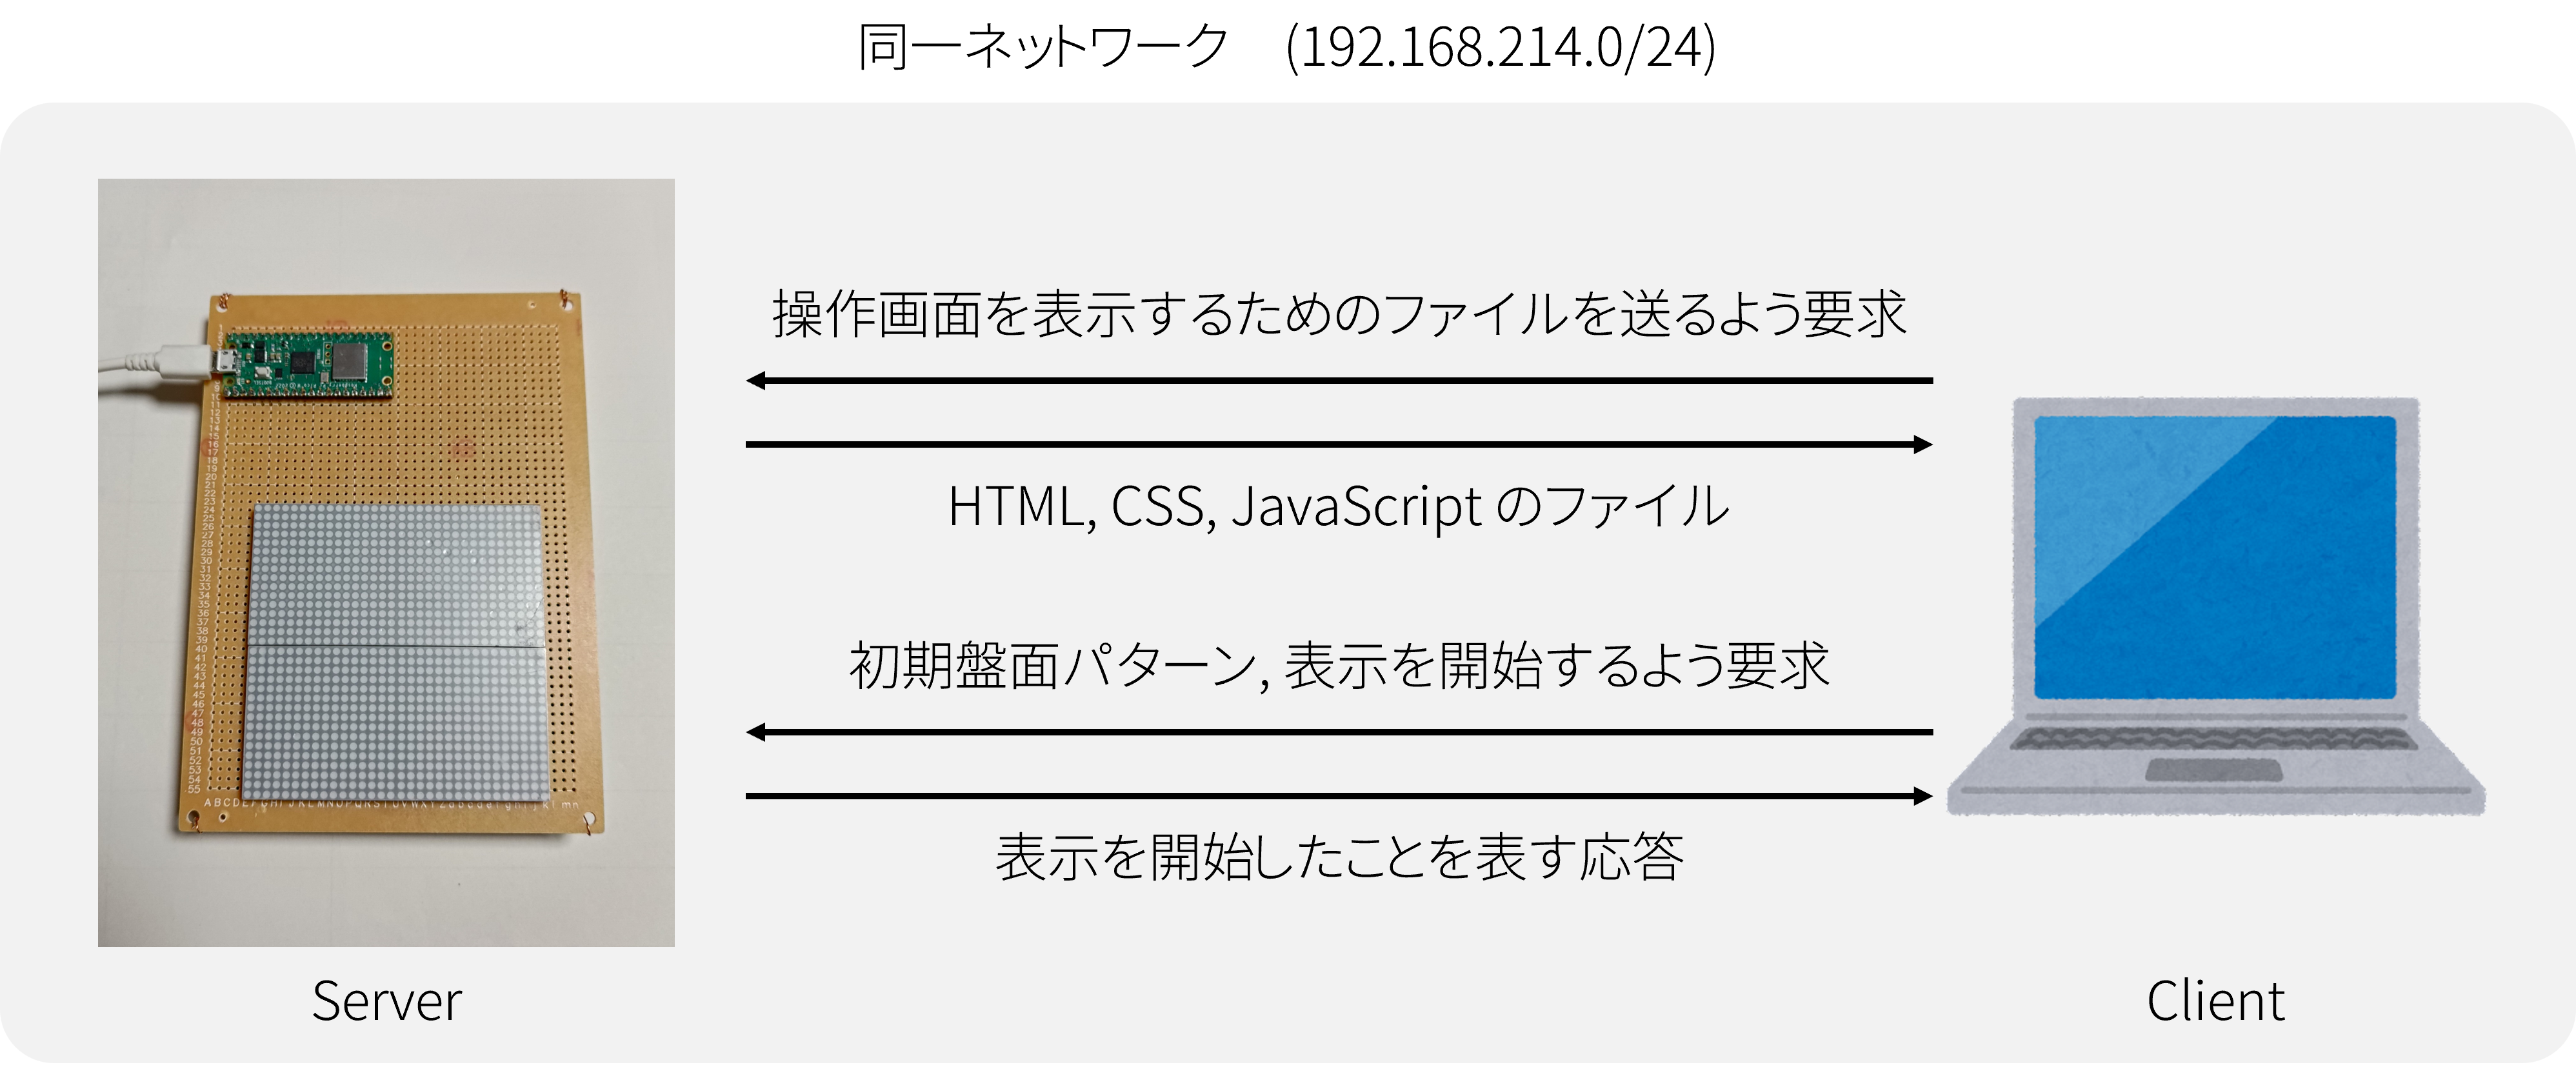
\includegraphics[width=120mm]{img/structure.png}
    \end{center}
    \caption{全体の構成図}
    \label{img:structure}
\end{figure}

\end{document}
